\documentclass{ws-fnl}

\usepackage{cite}
\usepackage{amsmath}
\usepackage{amssymb}
\usepackage{booktabs}
\usepackage{array}
\usepackage{graphicx}
\usepackage{url}

\let\trimmarks\relax

\begin{document}

\markboth{N. Krutikov and P. Lukianchenko}
{Detecting noise-induced transitions}

%%%%%%%%%%%%%%%%%%%%% Publisher's Area please ignore %%%%%%%%%%%%%%%
\catchline{}{}{}{}{}
%%%%%%%%%%%%%%%%%%%%%%%%%%%%%%%%%%%%%%%%%%%%%%%%%%%%%%%%%%%%%%%%%%%%

\title{A Controlled Benchmark for Statistical Detection of Noise-Induced
Transitions in Nonlinear Stochastic Dynamics}

\author{Nikita Krutikov}

\address{HSE University\\
Moscow, Russia}

\author{Petr Lukianchenko\footnote{Corresponding author.}}

\address{HSE University\\
Moscow, Russia\\
plukyanchenko@hse.ru}

\maketitle


\begin{abstract}
Noise-induced transitions are central to stochastic dynamics, but statistical
detection benchmarks often use externally inserted shifts. We study a
controlled alternative: trajectories of a nonlinear stochastic system where
events are labeled by transitions between state-space regions after simulation.
The task is therefore transition-time detection rather than ordinary
parameter-break detection. Classical tests, window-based procedures, and
learned detectors are evaluated under one protocol with independent training,
calibration, and test trajectories. In the frozen four-scenario benchmark,
classical homogeneity tests lead the sparse low-\(D\) white-noise case. Under
the primary 25-step tolerance, learned window-based detectors lead the evaluated
\(D=1.0\) cases and the strict-margin \(D=1.5\) white-noise case, whose ranking
is sensitive to wider tolerances. At \(D=1.0\) with white noise, Transformer has
the highest aggregate mean F1, but its paired difference from LSTM is not
statistically significant. A same-noise Transformer diagnostic shows that
noise-specific training alone does not produce a universal colored-noise neural
advantage under the evaluated pipeline.
\end{abstract}

\keywords{Change point detection; stochastic dynamics;
noise-induced transitions; colored noise; machine learning}

\section{Introduction}

Noise-induced transitions are a natural object of study in stochastic dynamics:
random fluctuations can move a trajectory between regions of state space even
when the underlying dynamical rule is fixed. From a statistical point of view,
the question is how accurately such transition times can be detected from an
observed series. Standard change point detection (CPD) simulations usually test
externally inserted shifts in mean, variance, or distribution; they do not cover
events generated by the stochastic process itself.

This paper studies that complementary setting. We generate trajectories from a
nonlinear stochastic dynamical system and label events by a fixed crossing rule
between state-space regions. The generating mechanism is not changed at the
event time; the label marks a transition of the trajectory between regions.
Thus the benchmark is designed for transition-time detection in stochastic
dynamics, not for structural-break detection in the usual parameter-change
sense. Rather than introducing a new detector or escape-rate theory, we use this
dynamics-generated process to compare existing detectors under fixed training,
calibration, testing, and matching rules.

The study makes four contributions. It defines a reproducible transition-time
benchmark with a specified generator, level-crossing labels, metadata, and
independent train/calibration/test splits. It evaluates classical tests,
segmentation and window-based procedures, and learned detectors under the same
matching protocol. It reports \(D\)-dependent rankings, including the
tolerance-sensitive \(D=1.5\) case, and uses a same-noise Transformer diagnostic
to delimit colored-noise neural-advantage claims.


\section{Related Work}

Change point detection (CPD) methods are usually grouped into online and
offline formulations; the offline setting used here estimates event locations
after the full series has been observed \cite{adams2007}. Surveys emphasize
that benchmark conclusions depend on detector assumptions, calibration,
post-processing, data generation, annotation, and matching rules
\cite{aminikhanghahi2017,truong2020,vandenburg2020}. Most simulations prescribe
the change structure directly, for example by placing shifts in a piecewise
signal or concatenating distinct segments
\cite{killick2012,fryzlewicz2014,gharghabi2019,ermshaus2023clasp}. Here the
labels come from a simulated stochastic trajectory: their number and spacing
are consequences of the dynamics and noise realization.

This distinction separates the benchmark from SDE-based detection models.
Recent work has used latent stochastic differential equations as a model class
for change point detection \cite{ryzhikov2023latent_sde_cpd}. Here the
stochastic dynamics are not the detector. They define the transition process on
which existing classical, window-based, and learned detectors are evaluated
under one fixed protocol.

The stochastic-dynamics motivation is rooted in noise-induced motion between
regions of state space. Classical work on random perturbations, escape
problems, and sample paths describes how fluctuations can drive transitions in
nonlinear systems \cite{kramers1940,freidlin1998,berglund2006}. Within
\textit{Fluctuation and Noise Letters}, noise-induced escape from the Lorenz
attractor has been studied as an escape problem in nonlinear dynamics
\cite{anishchenko2001fnl_escape}. Colored noise is also a natural part of this
setting rather than only a robustness stress test: FNL studies have examined
the role of colored noise in stochastic-system behavior
\cite{valenti2005fnl_colored}, and recent work has used deep learning to
characterize colored-noise time-series patterns
\cite{barauna2024fnl_colored_deep}. These papers motivate treating the
colored-noise diagnostic in this article as a boundary on neural claims, not as
a generic machine-learning add-on.

The compared methods cover standard CPD families: CUSUM-type, rank-based,
homogeneity, and structural-break tests
\cite{page1954,pettitt1979,alexandersson1986,buishand1982,chow1960};
segmentation and local-window methods
\cite{killick2012,harchaoui2009,liu2013}; and learned detectors trained from
labeled windows \cite{li2024deepcpd}. Because learned detectors use generated
labels, the benchmark keeps training, calibration, and test trajectories
independent.

\section{Data-Generating Process}

The benchmark generator is the discrete-time stochastic map
\begin{equation}
  x_{t+1}=x_t+\sin(x_t)\Delta t+\sqrt{D}\varepsilon_t,
\end{equation}
where the initial state is close to zero and \(\sin(x_t)\) gives a nonlinear
periodic drift. The innovation sequence \(\varepsilon_t\) is generated for a
fixed length, centered, and scaled to unit empirical variance when possible.
The map is motivated by stochastic dynamics, but it is not treated as a strict
Euler--Maruyama discretization of a continuous-time diffusion: the
implementation applies the \(\sqrt{D}\) factor shown above and does not add a
separate \(\sqrt{\Delta t}\) factor. Thus \(D\) controls the perturbation scale
of this discrete benchmark source.

Colored innovations are generated by Fourier-domain spectral shaping of a
Gaussian white sequence \cite{timmer1995,kasdin1995}. For a length-\(N\) draw,
the real Fourier transform \(Z_k\) is multiplied by
\begin{equation}
  a_c(f)=
  \begin{cases}
    1, & \text{white},\\
    f^{-1/2}, & \text{pink},\\
    f^{-1}, & \text{Brownian/red},\\
    f, & \text{violet},\\
    f^{1/2}, & \text{blue},
  \end{cases}
  \qquad f>0 .
\end{equation}
The zero-frequency component is not used for singular colored families. The
weights are normalized by their root mean square before the inverse transform;
the real sequence is then centered and scaled. Thus the innovation family
controls temporal correlation, not empirical variance scale.

\subsection{Transition Labels}

Change points in this benchmark are event labels, not parameter breaks in the
generator. Let \(L_t\) denote the integer level assigned to \(x_t/\pi\) by the
canonical level-mapping rule. The binary label at time \(t\) is one when
\(L_t \ne L_{t-1}\) and zero otherwise. The same stochastic map therefore
generates the whole path, while the level-crossing rule converts that path into
transition-time labels. A rule that directly recomputes \(L_t\) from \(x_t\)
would reproduce the annotation mechanism; it is not treated as a competing CPD
detector. The compared methods are evaluated as general-purpose detectors
applied to the trajectory without using the precomputed level sequence.

\begin{figure}[htbp]
  \centering
  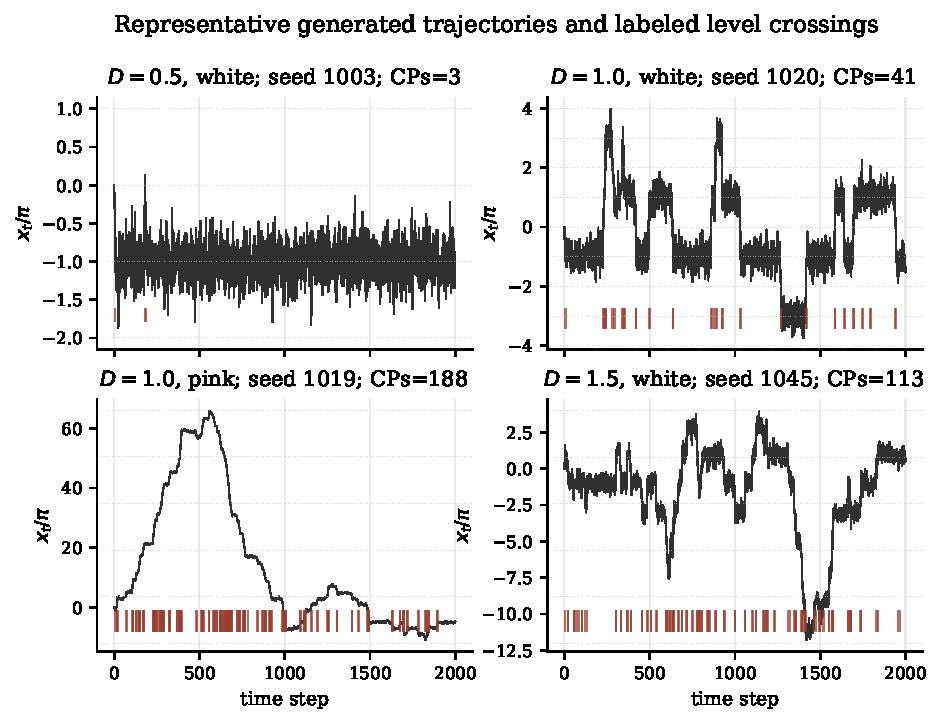
\includegraphics[width=\linewidth]{../assets/figures/fig01_generated_regime_examples.pdf}
  \caption{Representative trajectories and labeled level crossings under the
  four frozen benchmark scenarios. Red ticks indicate true labels; larger
  \(D\) or correlated innovations create denser transition neighborhoods.}
  \label{fig:generated-regime-examples}
\end{figure}

\subsection{Transition Properties}

The parameter \(D\) controls how often the trajectory leaves one level region.
In a diagnostic grid with \(\Delta t=1.0\), white innovations, length 10000,
and 30 series per setting, \(D=0.5\) produced 6.4 change points per series on
average, with mean positive holding time about 936 steps. For \(D=1.0\) and
\(D=1.5\), the corresponding values were about 197/50 and 576/17. Thus the
\(D=1.5\) case is dense relative to the 25-step matching tolerance and must be
read with the robustness check.

Because colored innovations change temporal correlation structure, colored-noise
comparisons are treated as separate experimental settings rather than direct
quantitative extensions of the white-noise cases.

The generator outputs \((x_{0:T}, y_{0:T})\), both of length \(T+1\), with
zero-based indexing. No-change cases use an all-zero label vector or an empty
change-point list. Reportable runs store the dataset source, generation
parameters \((T,\Delta t,D,\) noise type, seed\()\), and source path.


\section{Methods}

All detectors use a common interface: a one-dimensional series and seed are
mapped to zero-based predicted change points, optional per-timestep scores, and
method metadata. The shared evaluation layer then applies the same matching
margin and metrics to every method.

The classical group contains distributional and structural-break tests adapted
to the generated trajectories. Pettitt's rank-based test, SNHT, Buishand-type
homogeneity tests, and the Chow test provide interpretable baselines for level
or regression-structure changes. CUSUM is included as a sequential
mean-change detector derived from Page's cumulative-sum idea
\cite{page1954}. Additional segmentation-style baselines in the executable
registry include MDL, SWAB, Gaussian-process-based detection, and a Nyblom
test variant. These methods do not learn from the training split, but their
outputs are converted to the same change-point-list representation.

The learned group contains CatBoost, recurrent neural detectors, and a
Transformer detector. All learned detectors operate on normalized sliding
windows and return a local probability or logit for the window centre. Dense
scores are then thresholded and converted to change-point lists by
non-maximum suppression (NMS). The final benchmark configuration is summarized in
Table~\ref{tab:learned_method_configs}; the neural detectors are trained on
all five innovation families with \(D\) sampled from \([0.2,1.0]\) and
\(\Delta t \in \{0.5,1.0,2.0\}\).

\begin{table}[t]
\centering
\caption{Final learned-detector configurations used in the benchmark.}
\label{tab:learned_method_configs}
\small
\setlength{\tabcolsep}{3pt}
\begin{tabular}{@{}p{0.14\linewidth}p{0.08\linewidth}p{0.48\linewidth}p{0.22\linewidth}@{}}
\toprule
Method & Window & Architecture & Test post-processing \\
\midrule
CatBoost & 50 & 14 statistical window features; 500 trees, depth 6, learning rate 0.05 & threshold 0.57; NMS 50 \\
LSTM & 100 & two LSTM layers, hidden size 256, dropout 0.2; linear logit head & threshold 0.15; NMS 10 \\
GRU & 100 & two GRU layers, hidden size 128, dropout 0.2; linear logit head & threshold 0.15; NMS 10 \\
Transformer & 100 & \(d_{\mathrm{model}}=256\), 8 heads, 6 encoder layers, feed-forward size 512, dropout 0.1; mean pooling and linear logit head & threshold 0.15; NMS 10 \\
\bottomrule
\end{tabular}
\end{table}

The comparison separates method-specific scoring from shared evaluation. Only
final predicted change-point lists and, when available, dense score arrays are
passed to metric computation.


\section{Experimental Protocol}

The experiments follow a fixed data-generation contract. The current manuscript
tables use \texttt{algoritms/data\_utils.py}, the executable mirror of the
notebook source. Run metadata record length, time step, \(D\), noise type,
seed, dataset source, and source path. Allowed innovation families are white,
pink, Brownian, violet, and blue, each centered and scaled before entering the
map.

The benchmark uses independent generated trajectories, not timestep-level
splits: training seeds \(0\)--\(99\), calibration seeds \(5000\)--\(5019\), and
test seeds \(1000\)--\(1049\). The four frozen test scenarios are \(D=0.5\)
white, \(D=1.0\) white, \(D=1.0\) pink, and \(D=1.5\) white, all with length
2000 and \(\Delta t=1.0\).

Methods that require fitting use only the training split; thresholds and other
selection decisions are tuned on calibration data and frozen before test
evaluation. Classical methods are evaluated under the same matching and metric
definitions as learned detectors.

Change points are indexed from zero. The primary benchmark counts a predicted
change point as a match when it lies within 25 timesteps of an unmatched true
change point. This margin is an evaluation tolerance rather than a detector
hyperparameter, and is distinct from the non-maximum-suppression distance used
inside some learned detectors. The matching is one-to-one within a series. The
reported metrics are precision, recall, F1 score, and mean absolute
localization error for matched detections. For methods that return dense
scores, ROC-AUC and PR-AUC are also reported. When a method detects no change
points, its prediction is represented by an empty list rather than a missing
value.

\subsection{Choice of Matching Margin and Robustness}

The primary margin of 25 timesteps matches the frozen benchmark outputs used
for the main leaderboard. To check whether the qualitative conclusions depend
on this tolerance, all methods were rerun with frozen weights and unchanged
post-processing, and the same predictions were evaluated at matching margins
25, 50, and 100. This check is especially important for the \(D=1.5\) scenario,
where the diagnostic mean holding time is shorter than the primary matching
tolerance. No model was retrained in this robustness pass.
Table~\ref{tab:matching-margin-robustness} reports the leading method in each
scenario under each margin.

\begin{table}[t]
  \centering
  \caption{Leading mean F1 under alternative matching margins. The detector
  outputs and thresholds are fixed; only the evaluation tolerance changes.}
  \label{tab:matching-margin-robustness}
  \begin{tabular}{llll}
\toprule
Scenario & Margin 25 & Margin 50 & Margin 100 \\
\midrule
\(D=0.5\), white & SNHT 0.725 & SNHT 0.725 & SNHT 0.725 \\
\(D=1.0\), white & Transformer 0.698 & Transformer 0.723 & Transformer 0.790 \\
\(D=1.0\), pink & Transformer 0.566 & Transformer 0.589 & Transformer 0.610 \\
\(D=1.5\), white & Transformer 0.643 & CUSUM 0.666 & CUSUM 0.692 \\
\bottomrule
\end{tabular}

\end{table}

The low-\(D\) result is stable: SNHT remains the leading method for
\(D=0.5\) with white noise at all three margins. The two \(D=1.0\) scenarios
also preserve the same leading method, although wider margins increase the F1
of CUSUM. The \(D=1.5\), white-noise scenario is more sensitive to the chosen
tolerance: the Transformer detector leads under the primary, stricter margin,
whereas CUSUM leads when detections within 50 or 100 timesteps are counted as
matches. This indicates that the large-\(D\) ranking partly reflects
localization strictness, not only event-detection ability.

\begin{figure}[htbp]
  \centering
  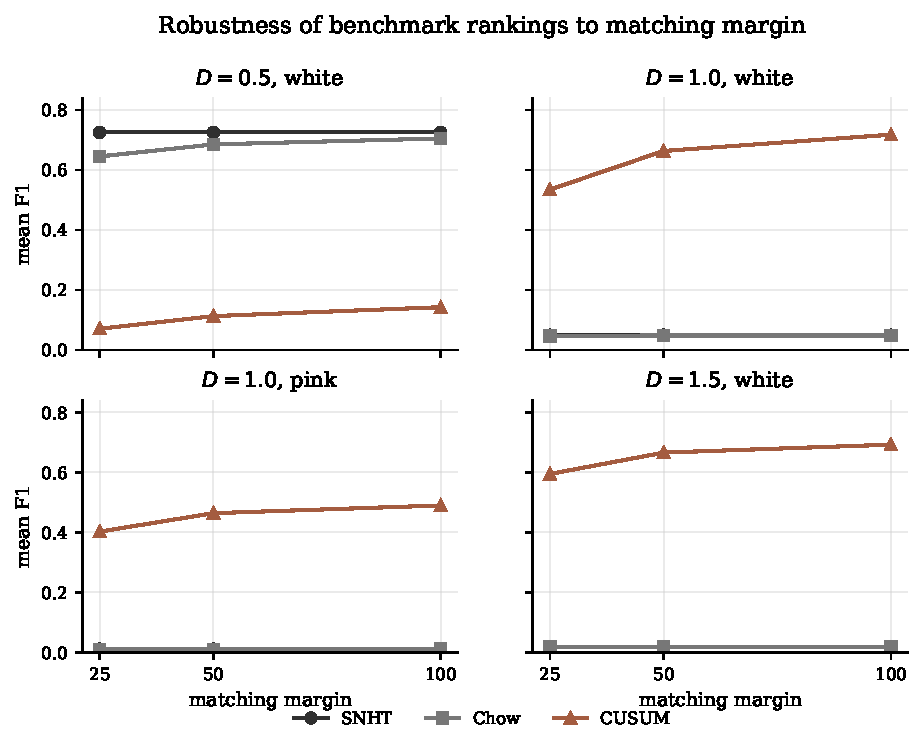
\includegraphics[width=\linewidth]{../assets/figures/fig03_matching_margin_robustness.pdf}
  \caption{Sensitivity of selected benchmark rankings to the matching margin.
  Detector outputs and post-processing are fixed; only the evaluation tolerance
  changes. The low-\(D\) and \(D=1.0\) conclusions are stable, while the
  \(D=1.5\) white-noise scenario shows the CUSUM--Transformer crossover under
  wider matching tolerances.}
  \label{fig:matching-margin-robustness}
\end{figure}



\section{Results}

This section reports the frozen four-scenario benchmark and the same-noise
Transformer diagnostic. Validation checks confirmed the expected test seeds
\(1000\)--\(1049\) and reproduced the stored scenario summaries from per-series
outputs under the primary 25-step matching margin. Table~\ref{tab:main-benchmark-top5}
reports the top five methods per scenario; full leaderboards are kept in the
reproducibility package.

\begin{table}[t]
  \centering
  \caption{Top five methods by mean F1 in each frozen benchmark scenario.
  Precision (P), recall (R), F1, mean absolute localization error (MAE),
  ROC-AUC (ROC), and PR-AUC (PR) are reported when available.}
  \label{tab:main-benchmark-top5}
  \begin{tabular}{llllllll}
\toprule
Scenario & Method & P & R & F1 & MAE & ROC & PR \\
\midrule
D=0.5, white & SNHT & 1.000 & 0.641 & 0.725 & 1.360 &  &  \\
D=0.5, white & Chow & 0.920 & 0.561 & 0.645 & 4.520 & 0.684 & 0.533 \\
D=0.5, white & GRU\_v2 & 0.322 & 0.230 & 0.253 & 3.180 & 0.918 & 0.551 \\
D=0.5, white & CatBoost & 0.355 & 0.213 & 0.243 & 4.280 & 0.650 & 0.211 \\
D=0.5, white & LSTM\_v2 & 0.237 & 0.209 & 0.207 & 2.320 & 0.866 & 0.424 \\
D=1, white & Transformer\_v2 & 0.774 & 0.641 & 0.698 & 3.560 & 0.815 & 0.799 \\
D=1, white & LSTM\_v2 & 0.840 & 0.569 & 0.675 & 3.350 & 0.813 & 0.811 \\
D=1, white & GRU\_v2 & 0.913 & 0.511 & 0.650 & 3.690 & 0.847 & 0.850 \\
D=1, white & CUSUM & 0.462 & 0.645 & 0.534 & 9.790 & 0.483 & 0.467 \\
D=1, white & CatBoost & 0.921 & 0.325 & 0.479 & 2.290 & 0.733 & 0.788 \\
D=1, pink & Transformer\_v2 & 0.916 & 0.410 & 0.566 & 3.330 & 0.896 & 0.972 \\
D=1, pink & GRU\_v2 & 0.987 & 0.384 & 0.551 & 2.610 & 0.922 & 0.981 \\
D=1, pink & LSTM\_v2 & 0.981 & 0.354 & 0.520 & 2.100 & 0.870 & 0.966 \\
D=1, pink & CUSUM & 0.794 & 0.270 & 0.402 & 7.500 & 0.474 & 0.783 \\
D=1, pink & CatBoost & 0.850 & 0.124 & 0.216 & 1.610 & 0.666 & 0.915 \\
D=1.5, white & Transformer\_v2 & 0.964 & 0.483 & 0.643 & 3.210 & 0.810 & 0.960 \\
D=1.5, white & LSTM\_v2 & 0.956 & 0.438 & 0.599 & 3.590 & 0.807 & 0.960 \\
D=1.5, white & CUSUM & 0.845 & 0.461 & 0.595 & 7.980 & 0.458 & 0.837 \\
D=1.5, white & GRU\_v2 & 0.969 & 0.278 & 0.429 & 3.280 & 0.806 & 0.959 \\
D=1.5, white & CatBoost & 0.991 & 0.206 & 0.341 & 2.100 & 0.828 & 0.968 \\
\bottomrule
\end{tabular}

\end{table}

\begin{table}[t]
  \centering
  \caption{Bootstrap confidence intervals for mean F1, computed by resampling
  independent test series.}
  \label{tab:bootstrap-f1-ci}
  \begin{tabular}{lll}
\toprule
Scenario & Method & Mean F1 [95\% CI] \\
\midrule
D=0.5, white & SNHT & 0.725 [0.650, 0.800] \\
D=0.5, white & Chow & 0.645 [0.555, 0.733] \\
D=0.5, white & GRU\_v2 & 0.253 [0.182, 0.329] \\
D=0.5, white & CatBoost & 0.243 [0.175, 0.313] \\
D=0.5, white & LSTM\_v2 & 0.207 [0.144, 0.273] \\
D=1, white & Transformer\_v2 & 0.698 [0.682, 0.714] \\
D=1, white & LSTM\_v2 & 0.675 [0.652, 0.696] \\
D=1, white & GRU\_v2 & 0.651 [0.630, 0.670] \\
D=1, white & CUSUM & 0.534 [0.518, 0.551] \\
D=1, white & CatBoost & 0.479 [0.469, 0.490] \\
D=1, pink & Transformer\_v2 & 0.566 [0.555, 0.577] \\
D=1, pink & GRU\_v2 & 0.551 [0.541, 0.561] \\
D=1, pink & LSTM\_v2 & 0.520 [0.508, 0.530] \\
D=1, pink & CUSUM & 0.402 [0.391, 0.413] \\
D=1, pink & CatBoost & 0.216 [0.209, 0.222] \\
D=1.5, white & Transformer\_v2 & 0.643 [0.631, 0.655] \\
D=1.5, white & LSTM\_v2 & 0.599 [0.586, 0.612] \\
D=1.5, white & CUSUM & 0.595 [0.586, 0.603] \\
D=1.5, white & GRU\_v2 & 0.429 [0.412, 0.446] \\
D=1.5, white & CatBoost & 0.341 [0.334, 0.348] \\
\bottomrule
\end{tabular}

\end{table}

\begin{figure}[htbp]
  \centering
  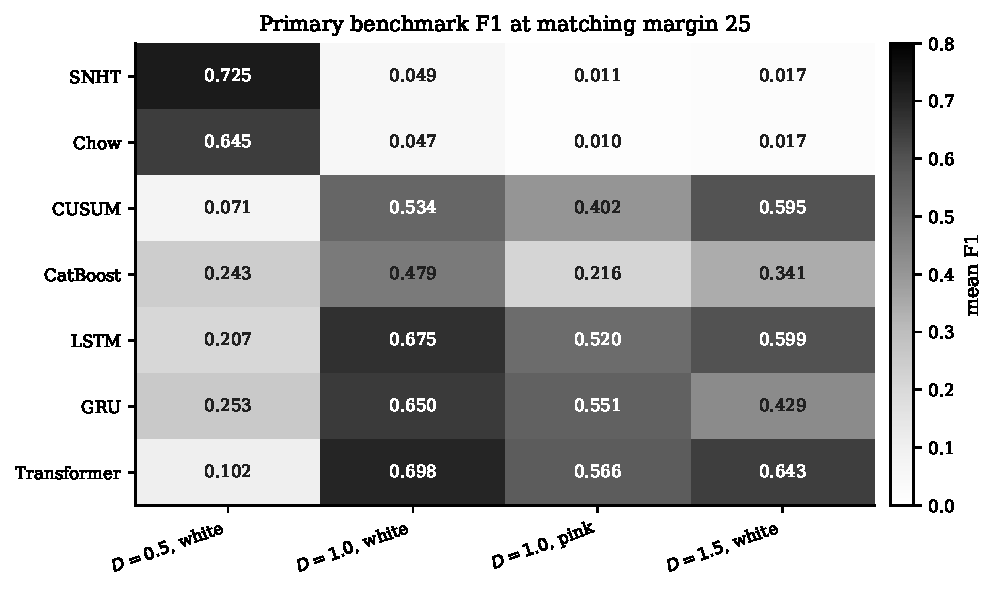
\includegraphics[width=\linewidth]{../assets/figures/fig02_primary_f1_benchmark.pdf}
  \caption{Primary benchmark F1 at the matching margin of 25 timesteps for the
  manuscript methods and frozen test scenarios. Classical tests lead in the
  sparse low-\(D\) setting; learned window-based detectors rank higher in the
  \(D=1.0\) and strict \(D=1.5\) evaluations.}
  \label{fig:primary-f1-benchmark}
\end{figure}

Table~\ref{tab:main-benchmark-top5} and Fig.~\ref{fig:primary-f1-benchmark}
separate the sparse low-\(D\) case from the larger-\(D\) cases. For \(D=0.5\)
with white noise, SNHT leads with mean F1 \(0.725\), followed by Chow at
\(0.645\); the strongest listed learned detector is far below this range. SNHT
also has low matched-event localization error, with MAE \(1.360\) timesteps.
For \(D=1.0\), learned window-based detectors rank higher: Transformer leads in
the white-noise and pink-noise scenarios, although the white-noise
Transformer--LSTM gap is qualified by the paired test below. For \(D=1.5\) with
white noise, Transformer leads under the primary 25-step margin, while LSTM and
CUSUM are close. The matching-margin robustness check shows that this ranking
is tolerance-sensitive: CUSUM overtakes Transformer when the evaluation
tolerance is widened to 50 or 100 timesteps.

\begin{figure}[htbp]
  \centering
  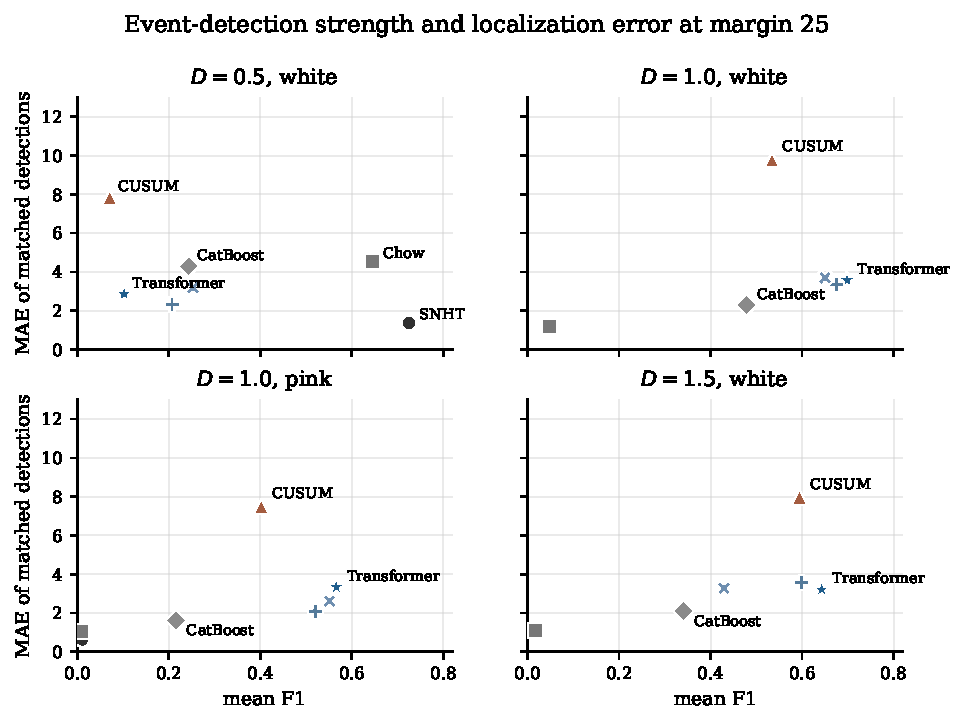
\includegraphics[width=\linewidth]{../assets/figures/fig04_f1_mae_tradeoff.pdf}
  \caption{Mean F1 and mean absolute localization error for selected methods at
  the primary matching margin. MAE is computed only for matched detections and
  should be read together with F1.}
  \label{fig:f1-mae-tradeoff}
\end{figure}

\begin{table}[t]
  \centering
  \caption{Paired Wilcoxon comparisons on per-series F1 for key method pairs.}
  \label{tab:paired-wilcoxon}
  \begin{tabular}{llllll}
\toprule
Scenario & A & B & Alt. & Mean F1 diff & p \\
\midrule
D=0.5, white & SNHT & Chow & greater & 0.080 & 0.0228 \\
D=0.5, white & SNHT & GRU\_v2 & greater & 0.472 & <0.0001 \\
D=1, white & Transformer\_v2 & CUSUM & greater & 0.164 & <0.0001 \\
D=1, white & Transformer\_v2 & GRU\_v2 & greater & 0.048 & <0.0001 \\
D=1, white & Transformer\_v2 & LSTM\_v2 & two-sided & 0.023 & 0.0937 \\
D=1, pink & Transformer\_v2 & CUSUM & greater & 0.164 & <0.0001 \\
D=1, pink & Transformer\_v2 & GRU\_v2 & two-sided & 0.015 & 0.0011 \\
D=1.5, white & Transformer\_v2 & CUSUM & greater & 0.048 & <0.0001 \\
D=1.5, white & Transformer\_v2 & LSTM\_v2 & two-sided & 0.044 & <0.0001 \\
\bottomrule
\end{tabular}

\end{table}

The paired tests in Table~\ref{tab:paired-wilcoxon} support the bounded ranking
claims. SNHT exceeds Chow and GRU in the \(D=0.5\), white-noise scenario. At
\(D=1.0\) with white noise, Transformer exceeds CUSUM and GRU, but the
Transformer--LSTM comparison remains close (\(p=0.0937\)). Under the primary
margin, Transformer exceeds CUSUM for \(D=1.0\) pink noise and \(D=1.5\) white
noise; the robustness pass qualifies the latter result because CUSUM improves
under wider tolerances.

\begin{figure}[htbp]
  \centering
  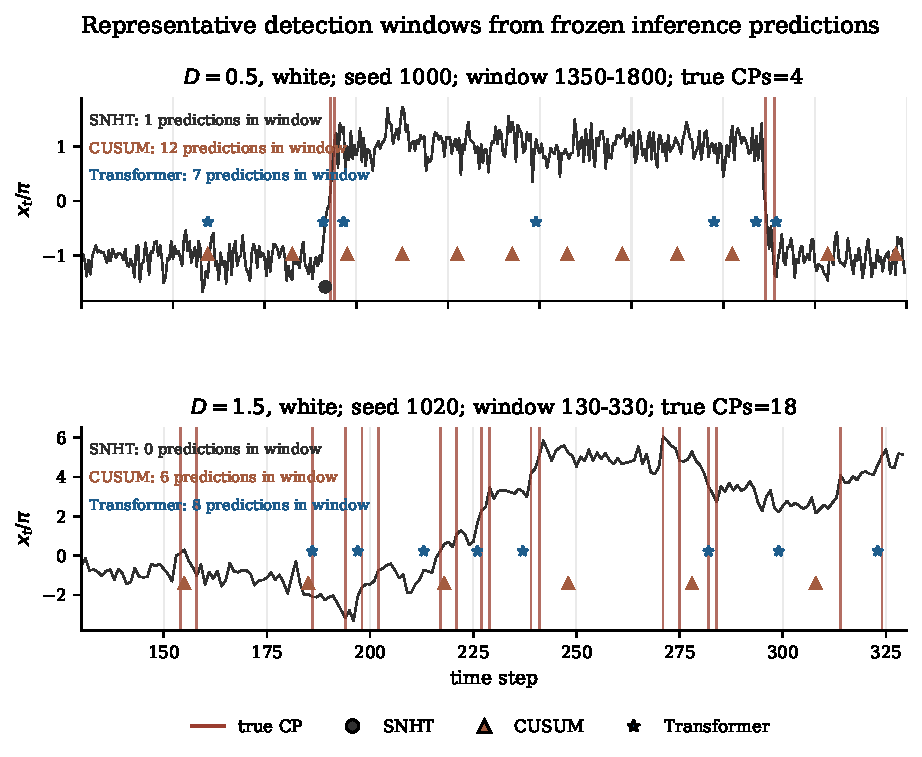
\includegraphics[width=\linewidth]{../assets/figures/fig05_detection_overlay.pdf}
  \caption{Representative detection windows. Vertical lines show true change
  points; markers show selected method predictions.}
  \label{fig:detection-overlay}
\end{figure}

\begin{table}[t]
  \centering
  \caption{Same-noise \(D=1.0\) diagnostic comparison against the best
  classical baseline on the same 50 test seeds.}
  \label{tab:same-noise-diagnostic}
  \begin{tabular}{llll}
\toprule
Noise & Transformer F1 & Classical F1 & Best classical method \\
\midrule
white & 0.586 & 0.663 & CUSUM \\
pink & 0.263 & 0.464 & CUSUM \\
brownian & 0.121 & 0.259 & CUSUM \\
blue & 0.160 & 0.523 & SNHT/Chow \\
violet & 0.078 & 0.793 & SNHT/Chow \\
\bottomrule
\end{tabular}

\end{table}

The same-noise experiment in Table~\ref{tab:same-noise-diagnostic} gives the
colored-noise boundary. Training and testing Transformer separately within each
\(D=1.0\) noise family still leaves it below the best classical baseline in all
five cases. Noise-specific Transformer training alone therefore does not support
a universal colored-noise neural-advantage claim under the evaluated pipeline.


\section{Discussion}

The benchmark should be read as regime-dependent evidence. In the \(D=0.5\)
white-noise scenario, labeled events are sparse and comparatively sharp in the
assigned state-space level, which aligns with homogeneity and structural-break
tests. SNHT and Chow therefore outperform the learned detectors in mean F1, and
SNHT also localizes matched events close to the labeled crossing. This is not a
general theorem about low-noise benchmarks; it is a result for the evaluated
stochastic map, labeling rule, universal-training setup, and matching protocol.
At \(D=1.0\) and under the strict \(D=1.5\) margin, local trajectory shape around
a crossing becomes more useful, so learned window-based detectors rank higher.
The \(D=1.0\) white-noise Transformer--LSTM comparison remains close, and the
\(D=1.5\) ranking is tolerance-sensitive. Thus the neural result is best read as
a strict-margin event-detection tradeoff, not as a universal claim about
transition-time precision.

The colored-noise results limit, rather than broaden, the neural claim. The
pink-noise scenario in the frozen benchmark is a transfer check for the
universally trained model, while the same-noise diagnostic tests whether
noise-specific Transformer training changes the conclusion. It does not: the
evaluated Transformer pipeline remains below the best classical baseline across
the five tested \(D=1.0\) noise families. For the present FNL framing, this is a
useful boundary. Temporal correlation structure is a separate benchmark
variable, and detector choice for colored noise should be validated directly
rather than extrapolated from the white-noise ranking.

The scope is deliberately narrow. The benchmark is one-dimensional, uses a fixed
main trajectory length, and evaluates four frozen scenarios rather than a dense
map over \(D\), \(\Delta t\), and noise families. Its conclusions are strongest
for trajectories from the same stochastic map with the same level-crossing
labels, split policy, calibration procedure, and matching rule. Alternative
state-space partitions, observation noise, latent-state settings, real sampling
mechanisms, or different detector calibration rules may change the ranking.
These boundaries are also what make the benchmark useful: it gives a controlled
reference point for detecting dynamics-induced transition events before moving
to less controlled data.


\section{Conclusion}

This paper presents a reproducible benchmark for comparing change point
detectors on dynamics-generated noise-induced transitions. The benchmark fixes
the stochastic map, labeling rule, train/calibration/test split, calibration
procedure, matching margin, and metrics, so that classical tests and learned
detectors are compared under one protocol.

The frozen four-scenario results show \(D\)- and noise-dependent rankings. In
the sparse \(D=0.5\) white-noise scenario, classical homogeneity tests lead.
Under the primary 25-step margin, learned window-based detectors lead the two
evaluated \(D=1.0\) scenarios and the strict-margin \(D=1.5\) white-noise
scenario. These conclusions are bounded: the \(D=1.5\) ranking is
tolerance-sensitive, and the \(D=1.0\) white-noise Transformer--LSTM gap is not
statistically significant in the paired test.

The same-noise diagnostic shows that noise-specific Transformer training alone
does not produce a universal colored-noise neural advantage under the evaluated
pipeline. The main contribution is therefore the controlled benchmark and the
evidence it provides for the evaluated stochastic-map scenarios. Future work
should test \(D\)- and noise-conditioned detectors, alternative label
partitions, and settings with noisy or latent observations.



\section*{Declaration of competing interest}
The authors declare no competing interests.

\section*{Data and code availability}
Code, configuration files, frozen benchmark outputs, and table/figure
reproduction scripts are available at \url{https://github.com/Nikkfh5/cpd}.
The repository is prepared as a versioned public release; a DOI-bearing archive
will be linked after archival deposition.

\section*{Funding}
This research did not receive any specific grant from funding agencies in the
public, commercial, or not-for-profit sectors.

\bibliographystyle{ws-fnl}
\bibliography{references}

\end{document}
